\documentclass[a4paper,11pt]{article}

\usepackage{amsmath}
\usepackage{amssymb}
\usepackage{listings}
\usepackage{color} %red, green, blue, yellow, cyan, magenta, black, white
\definecolor{mygreen}{RGB}{28,172,0} % color values Red, Green, Blue
\definecolor{mylilas}{RGB}{170,55,241}
%\usepackage{amsthm}
\usepackage{graphicx}
\usepackage{epstopdf}
\epstopdfsetup{update}
%\usepackage{caption}
%\usepackage{subcaption}

\newcommand{\ba}{\begin{array}}
\newcommand{\ea}{\end{array}}

\newcommand{\bea}{\begin{eqnarray}}
\newcommand{\eea}{\end{eqnarray}}

\newcommand{\bc}{\begin{center}}
\newcommand{\ec}{\end{center}}

\newcommand{\ds}{\displaystyle}

\newcommand{\bt}{\begin{tabular}}
\newcommand{\et}{\end{tabular}}

\newcommand{\bi}{\begin{itemize}}
\newcommand{\ei}{\end{itemize}}

\newcommand{\bd}{\begin{description}}
\newcommand{\ed}{\end{description}}

\newcommand{\bp}{\begin{pmatrix}}
\newcommand{\ep}{\end{pmatrix}}

\newcommand{\pd}{\partial}
\newcommand{\sech}{\mbox{sech}}

\newcommand{\cf}{{\it cf.}~}

\newcommand{\ltwo}{L_{2}(\mathbb{R}^{2})}
\newcommand{\smooth}{C^{\infty}_{0}(\mathbb{R}^{2})}

\newcommand{\br}{{\bf r}}
\newcommand{\bk}{{\bf k}}
\newcommand{\bv}{{\bf v}}

\newcommand{\gnorm}[1]{\left|\left| #1\right|\right|}
\newcommand{\ipro}[2]{\left<#1,#2 \right>}


\author{Matteo Polimeno}
\date{November $2^{nd}$, 2018}
\title{MATH693a\\
	Dr. Peter Blomgren\\
	HW03\\
	Trust Region Methods}
\begin{document}
\lstset{language=Matlab,%
		%basicstyle=\color{red},
		breaklines=true,%
		morekeywords={matlab2tikz},
		keywordstyle=\color{blue},%
		morekeywords=[2]{1}, keywordstyle=[2]{\color{black}},
		identifierstyle=\color{black},%
		stringstyle=\color{mylilas},
		commentstyle=\color{mygreen},%
		showstringspaces=false,%without this there will be a symbol in the places where there is a space
		numbers=left,%
		numberstyle={\tiny \color{black}},% size of the numbers
		numbersep=9pt, % this defines how far the numbers are from the text
		emph=[1]{for,end,break},emphstyle=[1]\color{red}, %some words to emphasise
		%emph=[2]{word1,word2}, emphstyle=[2]{style},    
}
\maketitle
\section*{Introduction}
In this assignment we were given the objective function:

\begin{align}
f(x) = 10(x_{2}-x_{1}^{2})^{2}+(1-x_{1})^{2} 
\end{align}

and asked to draw the contour lines of the quadratic model for it, assuming that for the Hessian of $f(x)$ would hold:

\begin{align}
B_{k} = \nabla^{2}f{({\bf x_{k})}}
\end{align}

and the family of solutions for the Trust Region subproblem.

\section*{Part 1}
In this section we will use $x_{0}=[0, -1]$ as our starting point, thus as the center of the trust region. We display the results of the iterations for some values of the trust region radius $D_{k}$, between $0$ and $2$.
We performed Cholesky Factorization on the Hessian to find the values of $\lambda$ (the diagonal elements of the Hessian) to use in order to shift the $2\times{2}$ matrix away from regions of non-definiteness (i.e. with any diagonal elements less than 0).\\
The table below shows the results in terms of number of iterations and the elapsed time necessary to converge to the optimal value for $\lambda$, given a maximum number of iterations fixed at 100 thousands.

\begin{center}
	\begin{tabular}{||c | c | c | c |||} 
		\hline
		$D_{k}$ & Iterations & Elapsed Time (sec) & Optimal $\lambda$ \\ [0.5ex] 
		\hline\hline
		0.5 & 13778 & 0.248767 & 20.0833\\ 
		\hline
		1 & 7201 & 0.146302 & 0.0227\\
		\hline
		1.5 & 100000 & 1.659368 & 19.7345\\
		\hline
		2 & 100000 & 1.721085 & 1.0984\\
		\hline
	\end{tabular}
\end{center}

We can immediately appreciate that for a trust-region radius $D_{k}\leq{1}$, we have a relatively fast convergence to an optimal value of $\lambda$. Whereas, for $D_{k}>1$, we do not have convergence for the point $x_{0}=[0,-1]$. Figure 1 below shows the contour of the model for such point, with the trust region and the step direction.

\begin{figure}[!ht]
	\centering
	\begin{tabular}{cc}
		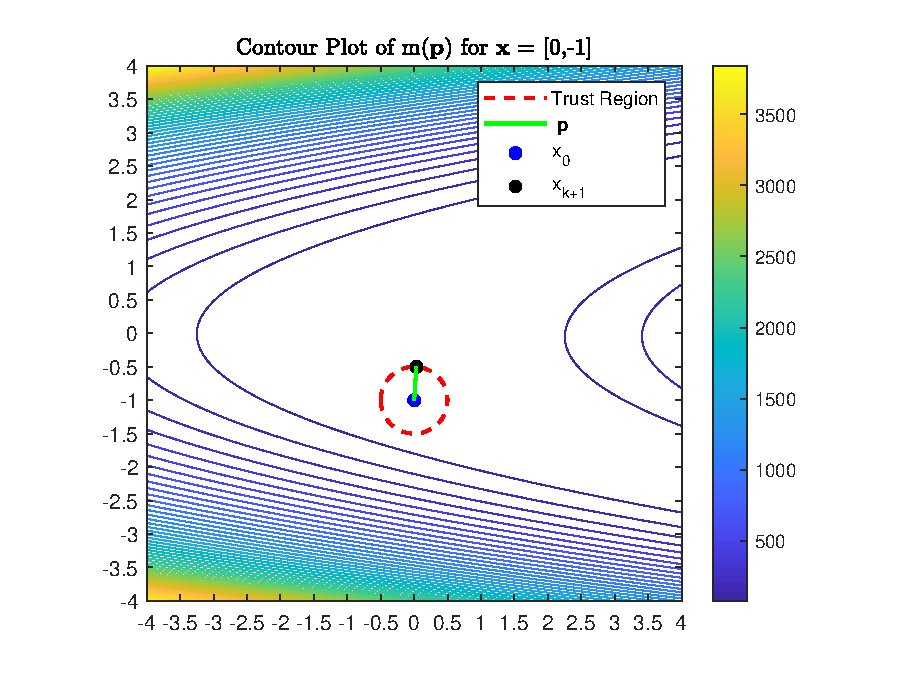
\includegraphics[width=.55\textwidth]{Trust_x0_Dk0p5} &\hspace{-25pt} 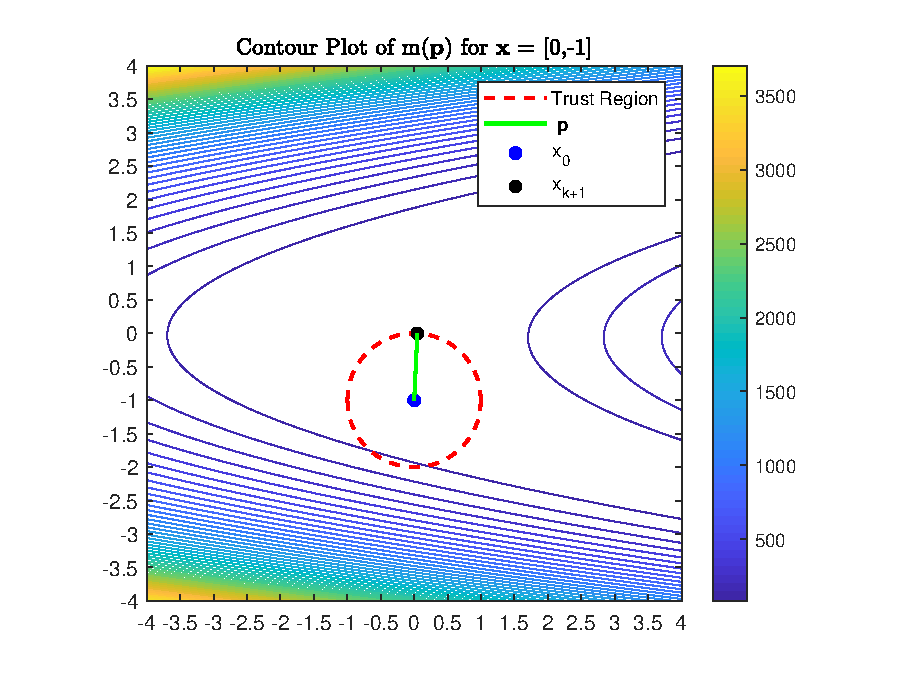
\includegraphics[width=.55\textwidth]{Trust_x0_Dk1} \\
		(a) & (b)\\
		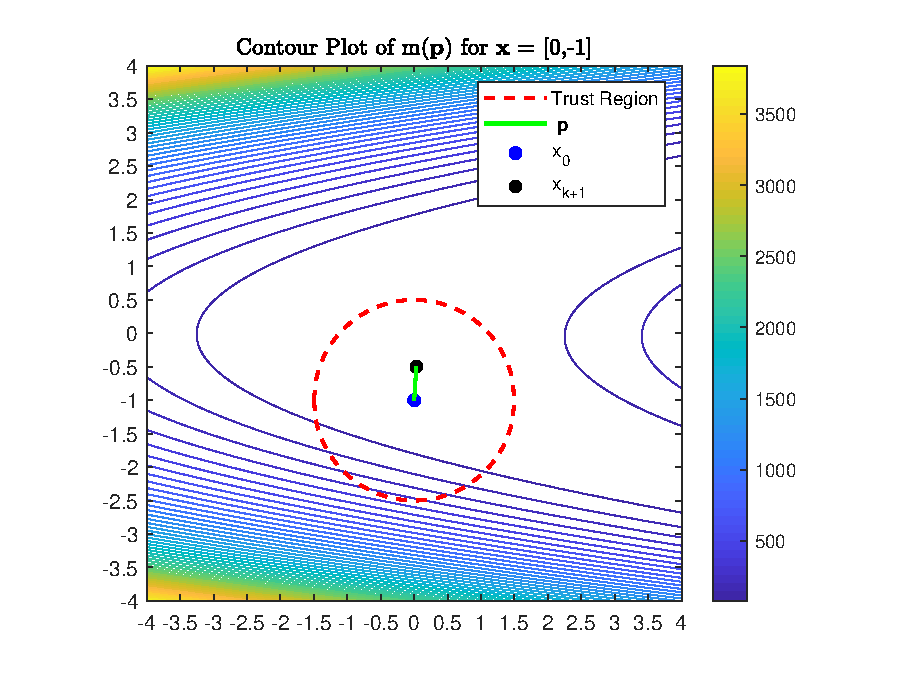
\includegraphics[width=.55\textwidth]{Trust_x0_Dk1p5} &\hspace{-25pt} 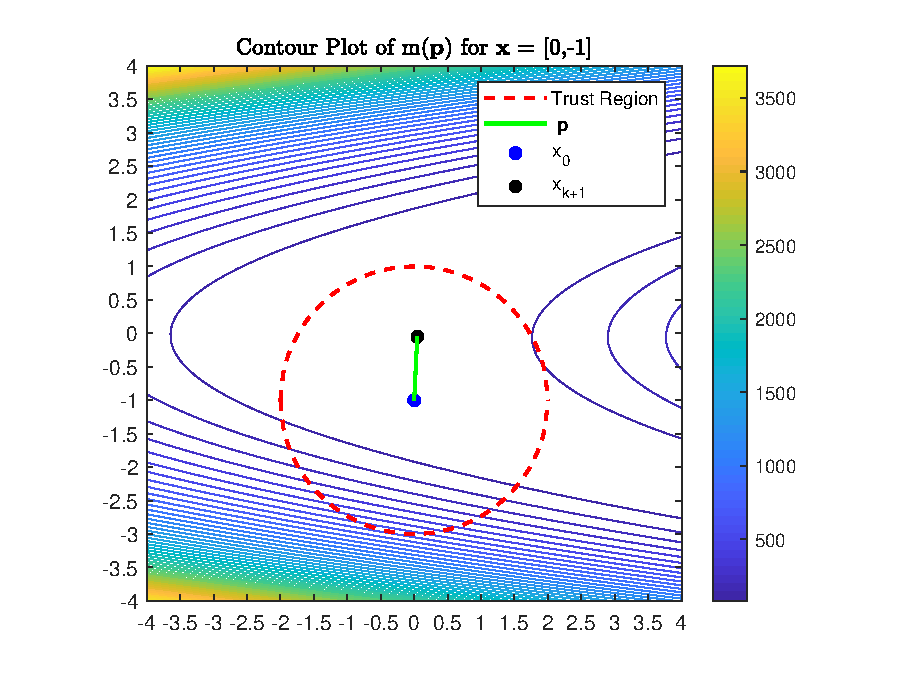
\includegraphics[width=.55\textwidth]{Trust_x0_Dk2} \\
		c) & d)\\
	\end{tabular}
	\caption{Trust Regions for different values of the radius $D_{k}$ for the starting point $x_{0}=[0,-1]$: a) $D_{k}=0.5$, b) $D_{k}=1$, c) $D_{k}=1.5$, d) $D_{k}=2$}
	\label{}
\end{figure}

We see that in Fig1a) and b), our lambda gives a step direction from the center of the trust region to its boundary, whereas in Fig1c) and d) we see that we stay well inside the region and the step length is much shorter than the trust region radius.

\section*{Part 2}
In this section we will use $x_{1}=[0, 0.5]$ as our starting point, thus as the center of the trust region. We display the results of the iterations for some values of the trust region radius $D_{k}$, between $0$ and $2$.
We performed Cholesky Factorization on the Hessian to find the values of $\lambda$ (the diagonal elements of the Hessian) to use in order to shift the $2\times{2}$ matrix away from regions of non-definiteness (i.e. with any diagonal elements less than 0).\\
The table below shows the results in terms of number of iterations and the elapsed time necessary to converge to the optimal value for $\lambda$, given a maximum number of iterations fixed at 100 thousands.

\begin{center}
	\begin{tabular}{||c | c | c | c|||} 
		\hline
		$D_{k}$ & Iterations & Elapsed Time (sec) & Optimal $\lambda$ \\ [0.5ex] 
		\hline\hline
		0.5 & 89318 & 1.440988 & 22.5324\\ 
		\hline
		1 & 23888 & 0.409682 & 20.0654\\
		\hline
		1.5 & 11193 & 0.230730 & 19.3529\\
		\hline
		2 & 6537 & 0.138706 & 19.0083\\
		\hline
	\end{tabular}
\end{center}

\begin{figure}[!ht]
	\centering
	\begin{tabular}{cc}
		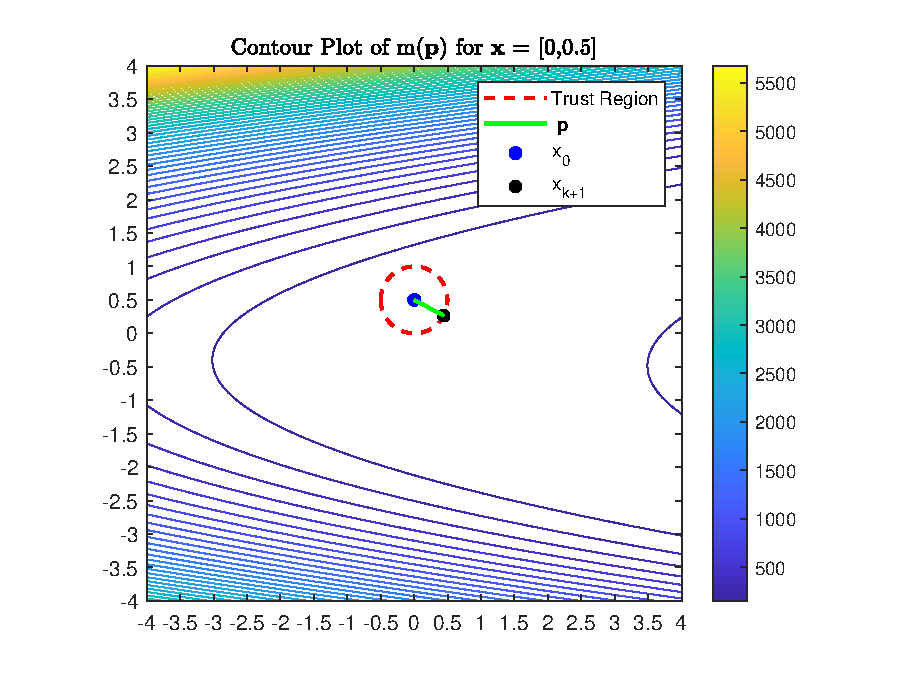
\includegraphics[width=.55\textwidth]{Trust_x1_Dk0p5} &\hspace{-25pt} 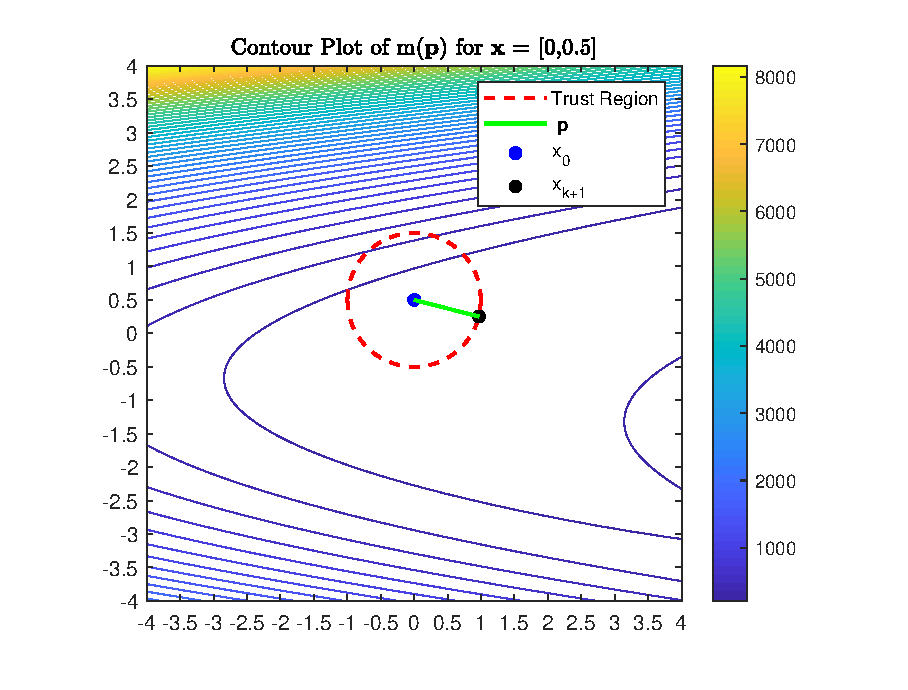
\includegraphics[width=.55\textwidth]{Trust_x1_Dk1} \\
		(a) & (b)\\
		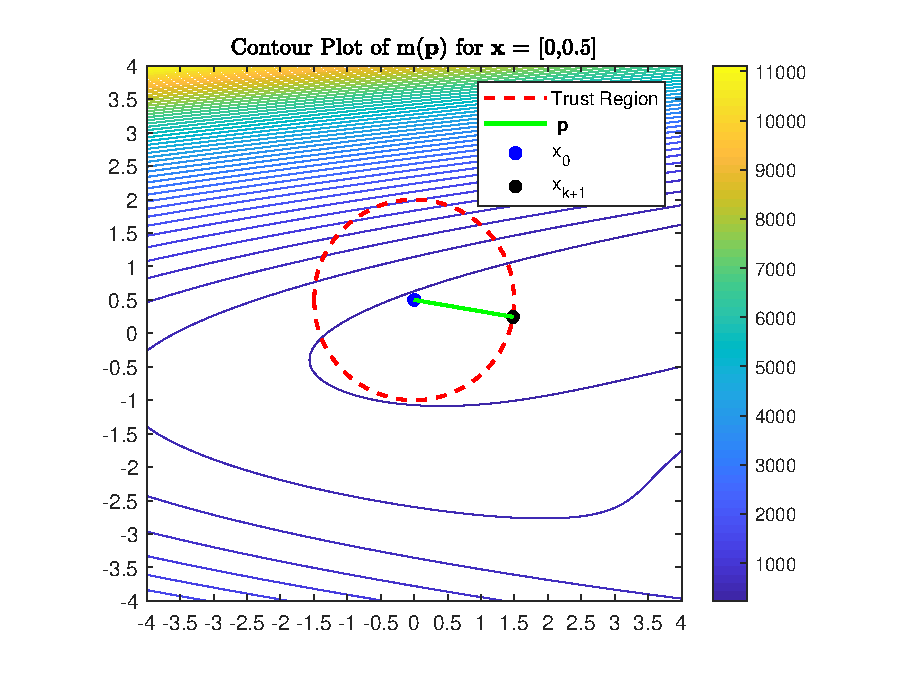
\includegraphics[width=.55\textwidth]{Trust_x1_Dk1p5} &\hspace{-25pt} 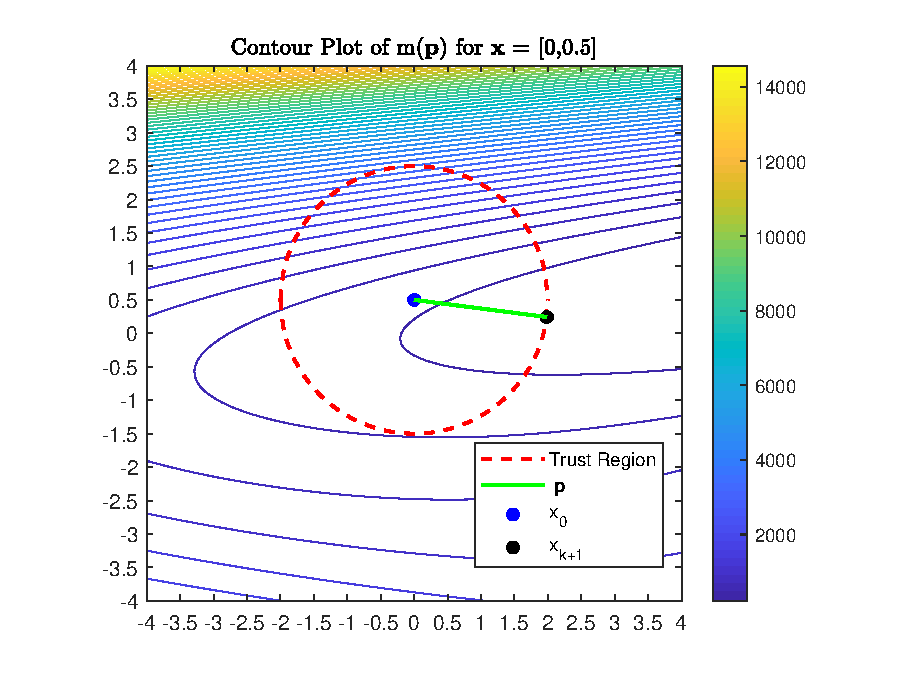
\includegraphics[width=.55\textwidth]{Trust_x1_Dk2} \\
		c) & d)\\
	\end{tabular}
	\caption{Trust Regions for different various of the radius $D_{k}$ for the starting point $x_{1}=[0,0.5]$: a) $D_{k}=0.5$, b) $D_{k}=1$, c) $D_{k}=1.5$, d) $D_{k}=2$}
	\label{}
\end{figure}

We can immediately appreciate that, in this case, for the four  trust-region radii $D_{k}s$ displayed, we have a relatively fast convergence to an optimal value of $\lambda$, with running time, number of iterations and $\lambda$ value that decrease as $D_{k}$ increases.\\
Below we plot the contour of the model $m({\bf p})$ for the given point, as well as the trust region and the step direction.

\clearpage
\section*{Appendix - Matlab Code}
\lstinputlisting{trust.m}

\end{document}